%\documentclass[preprint,tightenlines,showpacs,showkeys,floatfix,
%nofootinbib,superscriptaddress,fleqn]{revtex4} 
\documentclass[tightenlines,floatfix,nofootinbib,superscriptaddress,fleqn]{revtex4}  
%\documentclass[aps,epsfig,tightlines,fleqn]{revtex4}
\usepackage{kotex}
\usepackage[HWP]{dhucs-interword}
\usepackage[dvips]{color}
\usepackage{graphicx}
\usepackage{bm}
%\usepackage{fancyhdr}
%\usepackage{dcolumn}
\usepackage{defcolor}
\usepackage{amsmath}
\usepackage{amsfonts}
\usepackage{amssymb}
\usepackage{amscd}
\usepackage{amsthm}
\usepackage[utf8]{inputenc}
%\pagestyle{fancy}

\begin{document}

\title{\Large 2020년 2학기 물리학 II}
\author{김현철\footnote{Office: 5S-436D (면담시간 매주
    수요일-16:15$\sim$19:00)}} 
\email{hchkim@inha.ac.kr}
\affiliation{Hadron Theory Group, Department of Physics,
  Inha  University, Incheon 22212, Republic of Korea }
\date{Autumn Semester, 2020}

\maketitle

{\color{red} {\bf Due date:} 2020년 9월 14일  15:25-16:15 }
\vspace{1.cm}

\noindent \textbf{ 주의: \color{blue} 단 한 번의 부정행위도 절대
  용납하지 않습니다. 적발 시, 학점은 F를 받게 됨은 물론이고,
  징계위원회에 회부합니다. One strike out임을 명심하세요.} 
\\
\\

{\bf 학번:} \hspace{4cm}
{\bf 이름:} 

\section*{\large Quiz 5}
\noindent {\bf 문제 1 [20pt].} 반지름이 $r$이고 길이가 $L$인 원통형
구리 도선이 있다. 부피를 일정하게 유지한 채로 이 도선을 늘려 길이가 두
배가 되었다면, 저항은 처음의 몇 배가 되었는가? 
\newpage
{\color{gray} [문제 풀이 쪽]}
\newpage

\noindent {\bf 문제 2 [20pt].} 반지름이 $a$인 도체공을 중심이 같고
반지름이 $b$ ($b>a$)이고 비저항이 $\rho$인 물질로 만들어진 공을 감싸고
있다. 이 두 공 사이의 저항을 구하여라.  

\newpage
{\color{gray} [문제 풀이 쪽]} 
\newpage

\noindent {\bf 문제 3 [20pt].} 
저항값이 $R$인 저항이 달려 있는 단일고리
회로에 5.0 A의 전류가 흐르고 있다. 여기에 직렬로 저항이 $5.0\,\Omega$인
저항소자를 직렬로 회로에 연결하자 전류가 $4.0$ A로 낮아졌다. $R$ 값을
구하여라.   

\newpage
{\color{gray} [문제 풀이 쪽]}
\newpage

\noindent {\bf 문제 4 [20pt].} 
그림~\ref{fig:1}은 번개가 치는 날 나무 옆에 있으면 왜 안 되는지
보여준다. 나무에 낙뢰가 떨어지면, 나무껍질을 타고 번개전류가 흐른다.
그런데 번개전류가 나무껍질 중에서 물기가 없는 부분에 도달하면 전류 중
일부분이 습기가 높은 공기 중으로 새어나가 옆에 서 있는 사람에게로
흘러간다. 사람은 습도가 높은 공기에 비해 전도도가 훨씬 높아서
그렇다. 이때 나무와 사람 사이의 거리가 $d$이고, 사람의 키가 $h$라고
하면, 번개전류의 일부분이 나무에서 사람으로 $d$만큼 거리를 흐르고,
다시 사람을 따라 $h$만큼 높이를 흘러 바닥으로 간다고 하자. 만약에
$d/h=0.400$이고, 총전류는 $I=5\,000$ A라고 하면, 사람을 지나는 전류는
얼마인가? 

\begin{figure}[htp]
  \centering
  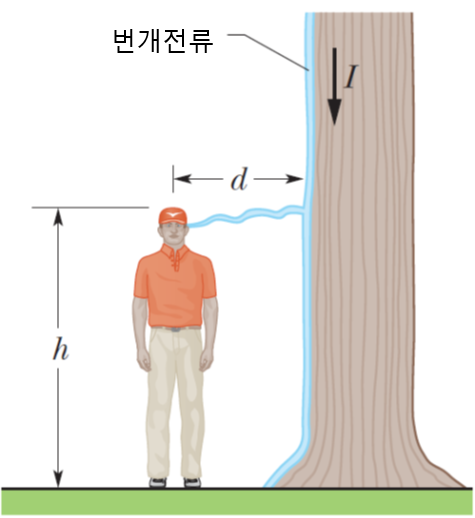
\includegraphics[scale=0.45]{qfig5-20220914-1.png}
  \caption{\textbf{문제 4}}
  \label{fig:1}
\end{figure}

\newpage
{\color{gray} [문제 풀이 쪽]}
\newpage

\noindent {\bf 문제 5 [20pt].} 
그림~\ref{fig:2}처럼 $a$와 $b$ 사이에 똑같이 생긴 저항 다섯 개가
연결되어 있을 때, 등가저항을 구하여라. 
\begin{figure}[htp]
  \centering
  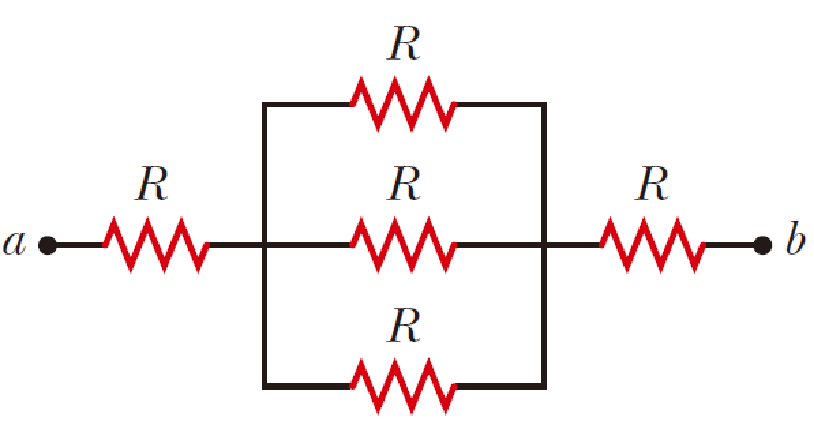
\includegraphics[scale=0.45]{qfig5-20220914-2.pdf}
  \caption{\textbf{문제 5}}
  \label{fig:2}
\end{figure}

\newpage
{\color{gray} [문제 풀이 쪽]}
\newpage
\end{document}